\documentclass[driverfallback=dvipdfmx,cjk]{beamer}

%\usepackage{bxdpx-beamer}% dvipdfmxなので必要
%\usepackage{pxjahyper}% 日本語で'しおり'したい
%\usepackage{minijs}% min10ヤダ
\renewcommand{\kanjifamilydefault}{\gtdefault}% 既定をゴシック体に

\AtBeginShipoutFirst{\special{pdf:tounicode 90ms-RKSJ-UCS2}}
%\AtBeginSection[]{
%    \frame{\tableofcontents[currentsection, hideallsubsections]} %目次スライド
%}
%\usepackage{amsmath,amssymb}
\usetheme{Antibes}
\usefonttheme{professionalfonts}
\usepackage{color}
\usepackage{mediabb}
\usepackage[absolute,overlay]{textpos}
%\usetheme{Madrid}
%
%\usecolortheme{albatross}
\useinnertheme{circles}
\setbeamertemplate{navigation symbols}{}
\setbeamertemplate{footline}[page number]
\setcounter{tocdepth}{2}


\title{XVA and its Greeks Calculation}
\author{森本 裕介}
\institute{三菱UFJ銀行}
\date{2018/11/23 - 11/25 \\ 数理ファイナンス合宿セミナー}
%%%%%% TEXT START %%%%%%
\begin{document}
\begin{frame}
\titlepage
\end{frame}

\begin{frame}\frametitle{Contents}
\begin{itemize}
    \item Definition of XVA
    \item Calculation of XVA
    \item Greeks calculation of XVA
\end{itemize}
\tableofcontents
\end{frame}

\section{Definition of XVA}
\subsection{Introduction}
\begin{frame} \frametitle{Definition of XVA}
    \begin{itemize}
        \item $V$ : 従来のデリバティブの価値
            \begin{itemize}
                \item Counter party risk(自社のクレジットリスク) を考慮しない
                \item 担保を勘案しない(Variation margin, Initial Margin)
                \item 自社のFunding コストを考慮しない
            \end{itemize}
        \item $\hat{V}$ : 上記に付随する金利のスプレッド, Cash flowを勘案したデリバティブの価値
    \end{itemize}
    $$\hat{V} = V + \sum_{X=C, D, F, M, ...} XVA$$
    \begin{itemize}
        \item CVA: counterparty credit risk adjustment
        \item DVA: Own credit risk adjustment
        \item FVA: Funding cost
        \item MVA: Margin cost
    \end{itemize}
\end{frame}

\begin{frame}
        $\hat{V}$の導出には色々なやり方があり、それに応じてXVAの表現にも色々な流派がある。
        そもそも、XVAの分け方は当然色々なものがあり、各社マネージのしやすさに応じて自社独自の
        コストの仕分けを行なっている。
        \begin{itemize}
            \item Piterburg
            \item Burgard and Kjaer
            \item Albanese and Andersen
            \item Fuji and Takahashi
            \item Takada
        \end{itemize}
\end{frame}

\begin{frame} \frametitle{Semi-Replication Theory }
    Burgard-Kjaer
    \begin{itemize}
        \item $S$ : Spot asset price \ 
        $ dS = \mu(t, S)Sdt + \sigma_s S dW_s $
        \item $r$ : risk free rate \ 
        $dr = \mu_r(t, r)dt + \sigma_r(t, r) dW_r$
        \item $P_r$: default free bond : $dP_r = rdP_r dt$
        \item $P_c, P_F$: counterpraty and bank bond 
        $$dP_* = r_* P_*(t-) dt - (1-R_*) P_*(t-) dJ_*, *=c,F$$
        \item $\beta_{*}$ : repo account \  $d\beta_{*} = r_* \beta_* dt, * = S, r, c, F$
        \item $r_* = r + s_*, \ s_* = (1-R_*)\lambda_*, \ *= c, F$
        \item $C = C_v + C_i$ : collateral (Variation margin, initial margin)
    \end{itemize}


\end{frame}

\begin{frame}
Bank から見たDerivativeの価値 $\hat{V}$
   $$\hat{V} = \hat{V}(t, r, S, J_F, J_c), $$
   $$ \hat{V}(T, r, S, 0, 0) = H(r, S),$$
   $$\hat{V}(t, R, S, 1, 0) = g_F, \hat{V}(t, R, S, 0, 1) = g_c.$$
 Hedging portfolio value $\Pi$
$$\Pi = \delta_s S + \delta_c P_c + \delta_r P_r + \delta_F P_F + \alpha_s\beta_s + \alpha_c \beta_c + \alpha_r \beta_r - C,$$
   $$ \Pi = \hat{V}.$$
   Hedge assetのRepo調達を仮定 
   $$\delta_s S + \alpha_s \beta_s = 0, $$
   $$\delta_c P_c + \alpha_c \beta_c = 0, $$
   $$\delta_r P_r + \alpha_r \beta_r = 0. $$
   Funding condition
   $$\hat{V} + \delta_F P_F - C = 0.$$

\end{frame}

\begin{frame}
    Semi-Replication 1: 自社のdefault risk意外を全てhedge
   \begin{align*}
    &d(\hat{V} + \Pi)\\
    = &\textcolor{blue}{\{ (\frac{\partial }{ \partial t} + \mathcal{A}) \hat{V} + r_F\delta_FP_F + \lambda_c(g_c - \hat{V}) -r_vC_v - r_iC_i \}}dt\\
    &  + \epsilon_h d J_B  
   \end{align*}
   $$ \hat{V}= V_{c_v} + CVA + FVA + MVA $$
   \begin{align*}
    &CVA = -E[\int_0^T \lambda_c(t) D^{r_F + \lambda_c}(V_{c_v}-g_c) \ dt]\\
    &FVA = -E[\int_0^T (r_F - r_{c_V}) D^{r_F + \lambda_c}(V_{c_V}-g_c) \ dt]\\
    &MVA = -E[\int_0^T (r_F - r_{c_i}) D^{r_F + \lambda_c}C_i \  dt]
   \end{align*}
\end{frame}

\begin{frame}
    FVA は自社のdefault riskを完全にhedgeできないことから出てくる
   \begin{align*}
    &FVA = DVA + FCA, \\
    &DVA = -E[\int_0^T \lambda_B(t) D^{r_F + \lambda_c}(V_{c_v}-g_B) \ dt]\\
    &FCA = -E[\int_0^T \lambda_B(t) D^{r_F + \lambda_c}\epsilon_h(t) \ dt].
   \end{align*}
   FVAに関する様々な議論(Hull, White, Albanese, Andersen, Crepy, Duffie, etc.)
   \begin{itemize}
        \item PricingはFundingと切り離して行われるべきだ
        \item Modiliani-Millarの定理: 企業価値はFunding strategyに依存しない に矛盾
        \item Shareholder value, Firm Value
   \end{itemize}

\end{frame}

\begin{frame}
    Semi-Replication 2 : Martingale Part以外をすべてhedge
    \begin{align*}
    = &\textcolor{red}{\{ (\frac{\partial }{ \partial t} + \mathcal{A} -r ) \hat{V} + \lambda_B(g_B - \hat{V}) + \lambda_c(g_c - \hat{V}) } \\
    & \textcolor{red}{+(r-r_v)C_v + (r- r_i) C_i \}} dt\\
    &  + \epsilon_h (d J_B - \lambda_B dt) .
   \end{align*}
   $$ \hat{V}= V_{c_v} + CVA + DVA + VMVA + VMVA + IMVA$$
   \begin{align*}
    &CVA = -E[\int_0^T \lambda_c(t) D^{r + \lambda_B + \lambda_c}(V_{c_v}-g_c) \ dt]\\
    &DVA = -E[\int_0^T \lambda_B(t) D^{r + \lambda_B + \lambda_c}(V_{c_v}-g_B) \ dt]\\
    &VMVA = -E[\int_0^T (r - r_{c_V}) D^{r + \lambda_B + \lambda_c}(V_{c_v}-C_v) \ dt]\\
    &IMVA = -E[\int_0^T (r - r_{c_i}) D^{r + \lambda_B + \lambda_c} C_i \  dt]
   \end{align*}

\end{frame}

\section{XVAの計算法} 
\begin{frame}\frametitle{XVAの計算法}
    \begin{itemize}
        \item Counterpraty c に対するXVAは概ね以下のような計算になる.
            $$ \text{XVA}(c) = \sum_{j=1}^J E\left[\int_0^T Z(t)\left(\sum_{k \in N_j(c)}V_k(t)- C(t)\right)^{(+)} \ dt\right] $$
            \begin{itemize}
                \item $V_k(t)$ : 取引kのExposure($t$時点の時価)
                    $$ V_k(t) = E\left[ \sum_{t_i > t} F_k(t_i, X(t_i)) | \mathcal{F}_t\right]$$
                \item $N_j(c)$ : cとの取引契約はいくつかのNetting Set(CSA条件などによって)に分かれている。
                    $$Trade(c) = \cup_{j=1}^J N_j(c)$$ 
                \item $Z$ : discount, spread, hazard, recovery rate, etc.
                \item $T$ : Trade(c) に含まれる取引の最長満期
            \end{itemize}
    \end{itemize}
\end{frame} 

\begin{frame}
    実際の計算は大きく2つに大別される。
    \begin{itemize}
        \item Approximate Exposure function \\
            $V_k$を原資産の関数として、その関数系を計算する。
            $$ \tilde{V}_k: \bf{R}^N \rightarrow \bf{R},$$
            $$V_k(t) \approx \tilde{V}_k(X(t))$$

        \item Aggregation
            \begin{itemize}
                \item $\tilde{V}_k(X(t))$から、Collateral $\tilde{C}$を計算.
                \item collateral勘案後のExposureにspreadをかけて積分を実施.
                    $$ E\left[\int_0^T \left(\tilde{V}_k(X(t)) -\tilde{C(t)} \right) D(t)\ dt\right].$$
            \end{itemize}
    \end{itemize}
\end{frame}

\begin{frame}\frametitle{Collateral計算法}
    \begin{itemize}
        \item VM(Variation Margin)
            \begin{itemize}
                \item $H$: Threshold. Exposureがこの額を超えていないと担保なし。
                \item $M$: MTA(minimum transfer amount). 支払い担保の最低額。
                \item $\delta$: MPOR(mergin period of risk). Default時点と最後に担保が支払われた時点のバッファ期間. e.g. 14day.
            \end{itemize}
            $$ C(t) = \left(V(t- \delta) - H\right)^+ 1_{\{V(t-\delta)-H > M\}}$$
        \item IM(Initial Margin)
            \begin{itemize}
                \item MPOR期間のGap Riskをカバーする。e.g. 10day 99\% Var.
                \item CCP(central counter party)や、SIMM(standard initial margin model)
                    ごとにGreeksを使ったVarの近似公式が決められている。
                    $$IM(t) = \sum \phi_{i,j} \frac{\partial V(t)}{\partial X^i(t)} \frac{\partial V(t)}{\partial X^j(t)}$$
            \end{itemize}
    \end{itemize}
\end{frame}

\begin{frame} \frametitle{XVAの数値計算手法}
    \begin{itemize}
        \item 大量のrisk facotor, productの計算を同時に行う必要があるため(Netting), Monte-Carlo法が通常使われる。
        \item Exposure 計算にはAmerican Monte Carlo法が使われる。
            多くの場合、LSM(Least square monte carlo)が用いられる。
            $$ \tilde{V}(x) = \sum_{i=1}^n a_i \phi_i(x), \ \phi_i: \text{polynomial}.$$
        \item LSMのメリット
        \begin{itemize}
            \item 計算が高速かつ汎用的: modelや商品性によらず、一律に適応できる
            \item Dataがシンプルになる: 複雑な取引情報を多項式の係数で表現できる
            \item Nettingが容易: pathを発生させなくても、多項式の係数の和でnettingできる。
        \end{itemize}
    \item LSMのデメリット
        \begin{itemize}
            \item 近似精度の問題
        \end{itemize}
    \end{itemize}
\end{frame}

\begin{frame}\frametitle{Implicit method}
無担保の場合は、Exposureの近似精度の悪さを補う次のような手法がある。
$$ XVA = E\left[\int_0^T Z(t)\left(\sum_{k \in N_j(c)}V_k(t)\right)^+ \ dt\right] $$
$$ = E\left[ \int_0^T Z(t) \left(\sum_{k \in N_j(c)} F_k(t_k, X(t_k)) \right) 1_{\{\sum_{k \in N_j(c)} V_k(t) \ge 0 \}} \right] $$
$$\approx E\left[ \int_0^T Z(t) \left(\sum_{k \in N_j(c)} F_k(t_k, X(t_k)) \right) 1_{\{\sum_{k \in N_j(c)} \tilde{V}_k(t) \ge 0 \}} \right] $$
\begin{itemize}
    \item Exposureの近似は正負の符号判定のみに用いられる。
    \item 値がどんなに離れていても符号さえ正しければ、誤差は発生しない。
\end{itemize}
\end{frame}

\begin{frame}
    \begin{Theorem}
       hogehoge 
    \end{Theorem}
    
\end{frame}

\begin{frame}
    \begin{align*}
    |\hat{c}_1(\omega)-c_0| \leqq C_{p,\delta}L^{-\frac{3/2(1-\delta)^2}{2+(1+\delta)(\tilde{N}+1)\ell_0/2}},
    \end{align*}
    for any $\omega \in \Omega_{L}$ and $L \geqq 1$.
    If there exists $\gamma \in (0,1]$ such that
$$\int_0^T E^{\mu}[ 1_{| \sum_{k:T_k\geqq t_{i+1}} (P_{T_k-t}^{(k)}F_k)(\pi_k (X(t)))| \leqq \theta\} } ]dt =O(\theta^{\gamma}), \text{as} \ \theta \downarrow 0,$$
 \begin{align*}
 |\hat{c}_2(\omega)-c_0| \leqq C_{p,\delta}L^{-\frac{3(\gamma+1)(1-\delta)^2}{(\gamma+2)(2+(1+\delta)(\tilde{N}+1)\ell_0/2)}},
 \end{align*}
特に$\gamma = 1$の場合、
$$|\hat{c}_1 - c_0| \leqq C_{p,\delta}L^{-\frac{3(1-\delta)^2}{2(2+(1+\delta)(N+1)\ell_0/2)}}$$ 
$$|\hat{c}_2 - c_0| \leqq C_{p,\delta}L^{-\frac{3(1-\delta)^2}{2+(1+\delta)(N+1)\ell_0/2}}$$ 
\end{frame}

\begin{frame}
    \begin{figure}
        \includegraphics[scale=0.25]{exposureAll.pdf}
    \end{figure}
\end{frame}

\section{XVAのGreeks計算}
\begin{frame}\frametitle{XVA Greeksの種類}
    XVAは多くのMarket Sensitivity(Greeks)を持っている。
    \begin{itemize}
        \item IR
            \begin{itemize}
                \item 金利スワップ (JPY 6m roll IRS, 1Y, 2Y, ...)
                \item Tenor basis swap (JPY 3m roll IRS, JPY 3m roll IRS, ...)
                \item 通貨スワップ (USD LIBOR vs JPY LIBOR + $\alpha$)
            \end{itemize}
        \item IR Vol
            \begin{itemize}
                \item Option満期 $\times$ Swap Tenor
            \end{itemize}
        \item FX 
        \item FX Vol
        \item Infration Swap, CDS, etc.
    \end{itemize}
    基本的にはGreeks計算は有限差分法を使って求める。
    $$Greeks(\theta) = \frac{XVA(\theta+ \epsilon) - XVA(\theta - \epsilon)}{2 \epsilon} $$
\end{frame}

\begin{frame}\frametitle{XVA Greeks 計算Tecnnique}
愚直に差分を一つ一つ計算する以外に、以下のようなTechniqueが提案されている。
\begin{itemize}
    \item Freezing method
        \begin{itemize}
            \item $XVA(\theta +(-) \epsilon)$を計算する際に、Regressionの結果は$XVA(\theta)$のものを使い回す方法
            \item American Optionの計算時にはうまくいくらしい。
        \end{itemize}
    \item Automatic Differentiation
        \begin{itemize}
            \item 関数を関数を計算する際に、微分も同時に求められるような実装テクニック
            \item Neural Networkのパラメータにも広く利用されている(Back Propagation)
        \end{itemize}
\end{itemize}
\end{frame}

\subsection{Freezing法}
\begin{frame}\frametitle{Freezing法の検証 }
    \begin{itemize}
        \item Parameter: $\theta = x_0 \  or  \ \sigma$
        \item model : BS model :  $d X(t,\theta) = X(t,\theta) ( \mu dt + \sigma dW(t)), \ X(0,\theta) = x_0.$
        \item Pay off function :$ F(x) = (x - K_1)^+  - K_2. $
        \item Exposure: $$ V(x, \theta) = E[F(X(T, \theta)) |X(t, \theta) = x] \approx \tilde{V}(x), $$
        \item Approximated Exposure:  $\tilde{V}(x, \theta)\approx V(x, \theta)$
        \item EPE: $EPE(t) = E[V(X(t))^+] $
    \end{itemize}
    この設定の下、Delta $\frac{\partial}{\partial x} EPE(t)$, 
 Vega 
    $\frac{\partial}{\partial \sigma} EPE(t)$, 
を計算する。

\end{frame}

\begin{frame}

    $$Explicit =  \frac{\tilde{V}(X(t,\theta+\epsilon),  \theta) - \tilde{V}(X(t,\theta-\epsilon), \theta)}{2 \epsilon} $$
\end{frame}


\begin{frame}\frametitle{Explicit法を用いたFreezing method}
    \begin{table}[htb]
        \caption{Test result of Delta}
        \centering
        \begin{tabular}{lcr}
            \hline
            method & mean & stdev \\
            analytic & 5.19 & 0.13 \\
            Non Freezing & 5.53 & 0.13\\
            Freezing & 5.22 & 0.21
        \end{tabular}
    \end{table}
    \begin{table}[htb]
        \caption{Test result of Vega}
        \centering
        \begin{tabular}{lcr}
            \hline
            method & mean & stdev \\
            analytic & 1264.77 & 61.08\\
            Non Freezing & 1480.38 & 74.98\\
            Freezing & \textcolor{red}{522.30} & 60.15
        \end{tabular}
    \end{table}
        DeltaはFreezingしても誤差はほとんどないが、VegaはFreezingすると誤差がとても大きい
\end{frame}


\begin{frame}\frametitle{Test結果の分析(Explicit法)}
    $$ \frac{\partial}{\partial \theta} E[V\left(X(t, \theta ), \theta \right)^+ ] = E[ 1_{\{  V\left(X(t, \theta), \theta\right) \geqq 0 \} }  \frac{\partial}{\partial \theta} V\left(X(t, \theta) , \theta \right)] $$
    $$= E[ 1_{\{  V\left(X(t, \theta), \theta\right) \geqq 0 \} }  \left(\frac{\partial V}{\partial x_1} \left(X(t, \theta) , \theta \right)\frac{\partial X(t, \theta)}{\partial \theta}  + \frac{\partial V}{\partial x_2} \left(X(t, \theta) , \theta \right)\right) ] $$
    \begin{itemize}
        \item $\theta = x_0$ の場合、$\frac{\partial V}{\partial x_2} \left(X(t, \theta) , \theta \right) = 0$ なので, $\theta$変化後にRegressionを再度やる必要はなかった。
        \item $\theta = \sigma$ の場合、$\frac{\partial V}{\partial x_2} \left(X(t, \theta) , \theta \right) \ne 0$なので、$\theta$変化後にRegressionをやり直さないと大きな誤差が生じる
    \end{itemize}
    \textcolor{red}{一般にMarkov過程でモデル化された原資産の初期値パラメータに関するGreeksであれば、Freezingの誤差はないが、そうでない場合はFreezingにより誤差が生じうる。}
\end{frame}

\begin{frame}\frametitle{Implicit法を用いたFreezing method}
    \begin{table}[htb]
        \caption{Test result of Delta}
        \centering
        \begin{tabular}{lcr}
            \hline
            method & mean & stdev \\
            analytic & 5.19 & 0.13 \\
            Non Freezing & 5.16 & 0.12\\
            Freezing & 5.16 & 0.12
        \end{tabular}
    \end{table}
    \begin{table}[htb]
        \caption{Test result of Vega}
        \centering
        \begin{tabular}{lcr}
            \hline
            method & mean & stdev \\
            analytic & 1264.77 & 61.08\\
            Non Freezing & 1262.38 & 60.99\\
            Freezing & \textcolor{red}{1262.38 } & 60.99
        \end{tabular}
    \end{table}

\end{frame}

\begin{frame}
    Implicit methodを使った場合、DeltaもVegaもうまくいく理由の分析
    $$ \frac{\partial}{\partial \theta} E[F(X(T, \theta ) 1_{\{  V\left(X(t, \theta), \theta\right) \geqq 0\}}  ] = E[ \frac{\partial F}{\partial x}(X(T, \theta))
    \frac{\partial X(t, \theta)}{\partial \theta} ]$$
    $$+ E[ F(X(T, \theta ))\delta_0(V\left( X(t, \theta), \theta \right)) \frac{\partial V}{\partial x_2} \left(X(t, \theta) , \theta \right) ]$$
    第二項目がExposure関数自体の$\theta$に関する変動を含んだ式になっている。ただし、次のように変形すると$0$ になることがわかる。
    $$ \text{(第二項)} = E[ E[ F(X(T, \theta )) | \mathcal{F}_t] \delta_0(V\left( X(t, \theta), \theta \right)) \frac{\partial V}{\partial x_2} \left(X(t, \theta) , \theta \right) ]$$
    $$= E[ V(X(t, \theta ))\delta_0(V\left( X(t, \theta), \theta \right)) \frac{\partial V}{\partial x_2} \left(X(t, \theta) , \theta \right) ]=0.$$
\end{frame}

\subsection{Automatic Differentiation}
\begin{frame}
    Automatic Differentiationの仕組み
    \begin{itemize}
        \item 基本的な関数の合成を計算グラフで表現し、プログラム内にその構造を保持
        \item 基本的な関数の微分は既知なので、その関数もプログラムしておく
        \item 最終的に得られる関数は基本関数の合成なので、Treeをたどって、各ノードの微分を掛け合わせて行くことが、Chain ruleに対応しており、最終的なGreeksが求められる
    \end{itemize}
\end{frame}

\begin{frame}
    \begin{figure}
    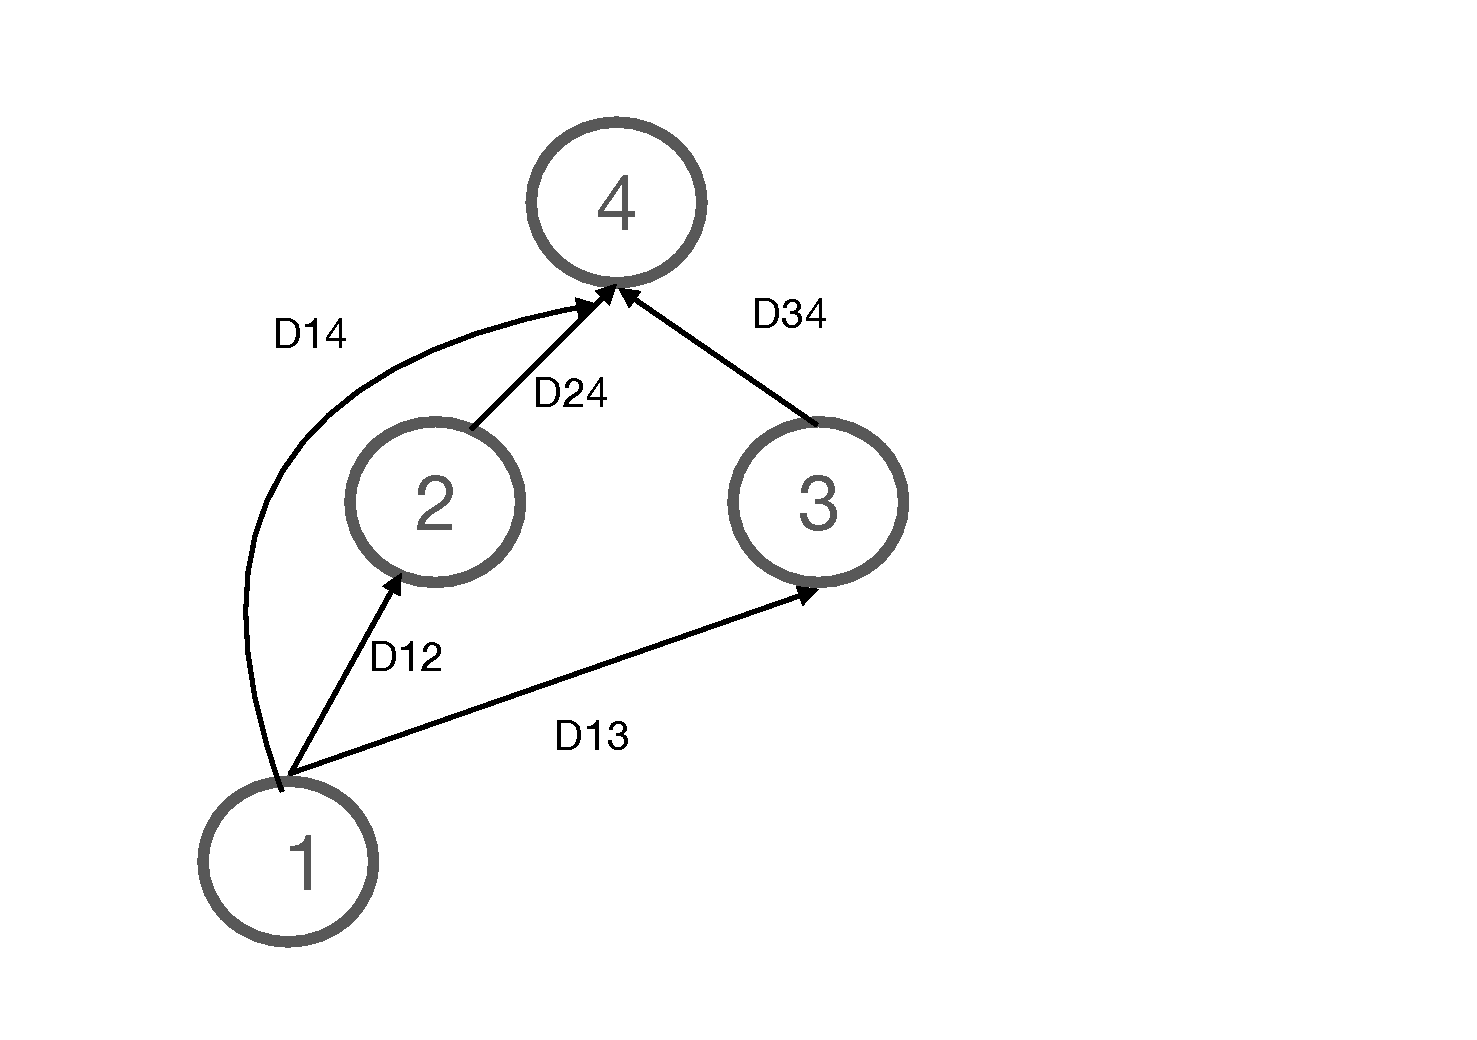
\includegraphics[scale=0.4]{AADImage.pdf}
    \end{figure}
    $$ \frac{d x_4}{d x1} = D14 + D12 * D24 + D13 * D34$$
\end{frame}

\begin{frame}\frametitle{XVA計算におけるADのメリット、デメリット}
    メリット
    \begin{itemize}
        \item 通常の値の計算の数倍(10未満?)で大量のGreeks計算が出来る。
        \item 真の関数の微分を実装しているので、差分法のようなバイアスがない。
    \end{itemize}
    デメリット
    \begin{itemize}
        \item 大量のメモリが必要
        \item On memory で一気通貫で計算しないと厳しい。途中で中間データを出力しながらだと、巨大なヤコビ行列を計算する必要が生じる。 
        \item 途中に滑らかでない関数が入ると一気に依存するポイントのGreeksがおかしくなる
        \item pathごとの微分を行なっていくので、熱核で積分して滑らかになる要素が含まれていない。
    \end{itemize}
\end{frame}

\begin{frame}
    AADの最近の進展
    \begin{itemize}
        \item Stochastic AAD
        \item MVAへの応用
        \item ccp
    \end{itemize}

\end{frame}


\end{document}
